\let\negmedspace\undefined
\let\negthickspace\undefined
\documentclass[journal]{IEEEtran}
\usepackage[a5paper, margin=10mm, onecolumn]{geometry}

\usepackage{tfrupee}
\setlength{\headheight}{1cm}
\setlength{\headsep}{0mm}

\usepackage{gvv-book}
\usepackage{gvv}
\usepackage{cite}
\usepackage{amsmath,amssymb,amsfonts,amsthm}
\usepackage{algorithmic}
\usepackage{graphicx}
\graphicspath{{figs/}}
\usepackage{textcomp}
\usepackage{xcolor}
\usepackage{txfonts}
\usepackage{listings}
\usepackage{enumitem}
\usepackage{mathtools}
\usepackage{gensymb}
\usepackage{comment}
\usepackage[breaklinks=true]{hyperref}
\usepackage{tkz-euclide}
\usepackage{listings}

\def\inputGnumericTable{}
\usepackage[latin1]{inputenc}
\usepackage{color}
\usepackage{array}
\usepackage{longtable}
\usepackage{calc}
\usepackage{multirow}
\usepackage{hhline}
\usepackage{ifthen}
\usepackage{lscape}

\begin{document}

\bibliographystyle{IEEEtran}

\title{1.6.29}
\author{AI25BTECH11014-Suhas}

{\let\newpage\relax\maketitle}

\renewcommand{\thefigure}{\theenumi}
\renewcommand{\thetable}{\theenumi}
\setlength{\intextsep}{10pt}

\numberwithin{equation}{enumi}
\numberwithin{figure}{enumi}
\renewcommand{\thetable}{\theenumi}

\section*{Question}
\vspace{0.5cm}
Show that the points $A = \myvec{2\\3\\-4}$, $B = \myvec{1\\-2\\3}$, and $C = \myvec{3\\8\\-11}$ are collinear.

\section*{Solution}
\vspace{0.5cm}
To prove that the points are collinear, we examine whether the vectors $\vec{B} - \vec{A}$ and $\vec{C} - \vec{A}$ are linearly dependent.

\subsection*{Step 1: Define the Points}
Let the position vectors be:
\begin{align}
\vec{A} &= \myvec{2\\3\\-4} \\
\vec{B} &= \myvec{1\\-2\\3} \\
\vec{C} &= \myvec{3\\8\\-11}
\end{align}

\subsection*{Step 2: Compute Direction Vectors}
We compute the vectors from point A to B and A to C:
\begin{align}
\vec{B} - \vec{A} &= \myvec{1\\-2\\3} - \myvec{2\\3\\-4} = \myvec{-1\\-5\\7} \\
\vec{C} - \vec{A} &= \myvec{3\\8\\-11} - \myvec{2\\3\\-4} = \myvec{1\\5\\-7}
\end{align}

\subsection*{Step 3: Form the Matrix}
We now construct a matrix $M$ whose rows are the vectors $\vec{B} - \vec{A}$ and $\vec{C} - \vec{A}$:
\begin{equation}
M = \myvec{-1 & -5 & 7\\1 & 5 & -7}
\label{eq:matrix}
\end{equation}

\subsection*{Step 4: Rank via Echelon Form}
To determine the rank of matrix $M$, we reduce it to **echelon form** using row operations.

First, swap $R_1$ and $R_2$ to make the leading entry positive:
\begin{equation}
\myvec{1 & 5 & -7\\-1 & -5 & 7}
\label{eq:swap}
\end{equation}

Next, eliminate the first entry of $R_2$:
\begin{equation}
R_2 \rightarrow R_2 + R_1 \Rightarrow
\myvec{1 & 5 & -7\\0 & 0 & 0}
\label{eq:echelon}
\end{equation}

\subsection*{Step 5: Echelon Matrix}
The resulting **echelon form** of matrix $M$ is:
\begin{equation}
E = \myvec{1 & 5 & -7\\0 & 0 & 0}
\label{eq:echelon_matrix}
\end{equation}

\subsection*{Step 6: Rank of the Matrix}
From equation \eqref{eq:echelon_matrix}, we observe that only one row is non-zero. Therefore, the rank of matrix $M$ is:
\begin{equation}
\text{Rank}(M) = 1
\label{eq:rank}
\end{equation}

\subsection*{Step 7: Conclusion}
Since the rank of the matrix formed by the vectors $\vec{B} - \vec{A}$ and $\vec{C} - \vec{A}$ is 1, the vectors are linearly dependent.  
Hence, the points $A$, $B$, and $C$ lie on the same line.  
\textbf{Therefore, the points are collinear.}

\newpage
\begin{figure}[h!]
   \centering
   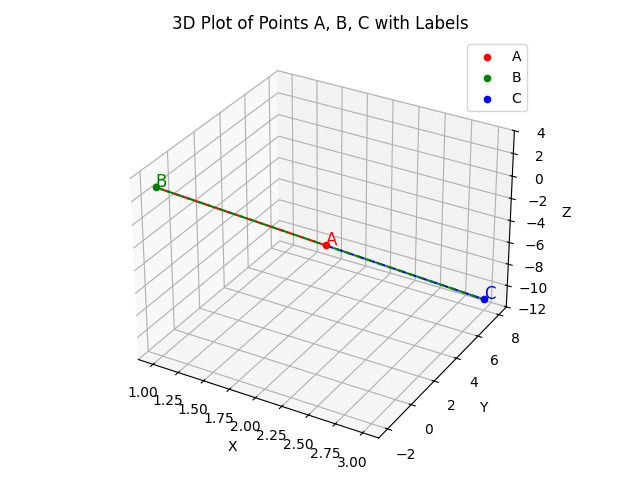
\includegraphics[width=1\linewidth]{figs/fig1.png}
   \caption{3D plot of points A, B, C showing collinearity}
   \label{}
\end{figure}

\end{document}

















